%%%%%%%%%%%%%%%%%%%
%%% 2023-08-22 %%%%
%%%%%%%%%%%%%%%%%%%
\section{La plataforma ROS (2023-08-22)}
\begin{frame}\frametitle{La plataforma ROS}
  
\includegraphics[width=0.3\textwidth]{Figures/Ros_logo.png}
  \[\]
  \textbf{ROS (Robot Operating System) } es un \textit{middleware} de código abierto para el desarrollo de robots móviles.
  \begin{itemize}
  \item Implementa funcionalidades comúnmente usadas en el desarrollo de robots como el paso de mensajes entre procesos y la administración de paquetes.
  \item Muchos drivers y algoritmos ya están implementados.
  \item Es una plataforma distribuida de procesos (llamados \textit{nodos}).
  \item Facilita el reuso de código.
  \item Independiente del lenguaje (Python y C++ son los más usados).
  \item Facilita el escalamiento para proyectos de gran escala. 
  \end{itemize}
\end{frame}

\begin{frame}\frametitle{Conceptos}
  ROS se puede entender en dos grandes niveles conceptuales:
  \begin{itemize}
  \item \textbf{Sistema de archivos:} Recursos de ROS en disco
  \item \textbf{Grafo de procesos:} Una red \textit{peer-to-peer} de procesos (llamados nodos) en tiempo de ejecución.
  \end{itemize}
\end{frame}

\begin{frame}\frametitle{Sistema de archivos}
  \begin{columns}
    \begin{column}{0.5\textwidth}
      Recursos en disco:
      \begin{itemize}
      \item \textbf{Workspace:} carpeta que contiene los paquete desarrollados
      \item \textbf{Paquetes:} Principal unidad de organización del software en ROS (concepto heredado de Linux)
      \item \textbf{Manifiesto:} (\texttt{package.xml}) provee metadatos sobre el paquete (dependencias, banderas de compilación, información del desarrollador)
      \item \textbf{Mensajes (msg):} Archivos que definen la estructura de un \textit{mensaje} en ROS.
        \item \textbf{Servicios (srv):} Archivos que definen las estructuras de la petición (\textit{request}) y respuesta (\textit{response}) de un servicio. 
      \end{itemize}
    \end{column}
    \begin{column}{0.4\textwidth}
      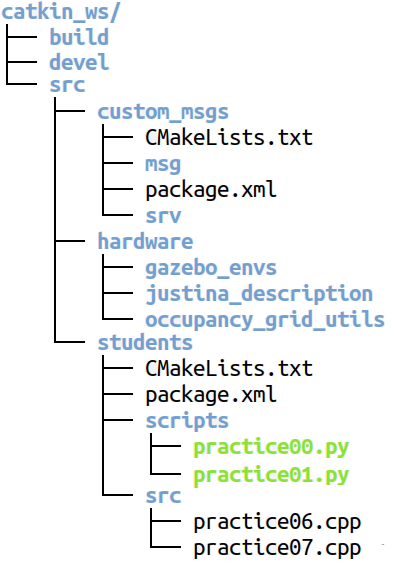
\includegraphics[width=\textwidth]{Figures/catkin_tree.png}
    \end{column}
  \end{columns}
\end{frame}

\begin{frame}\frametitle{Grafo de procesos}
  El grafo de procesos es una red \textit{peer-to-peer} de programas (nodos) que intercambian información entre sí. Los principales componentes del este grafo son:
  \[\]
  \begin{columns}
    \begin{column}{0.5\textwidth}
      \begin{itemize}
      \item master
      \item servidor de parámetros
      \item nodos
      \item mensajes
      \item servicios 
      \end{itemize}
    \end{column}
    \begin{column}{0.5\textwidth}
      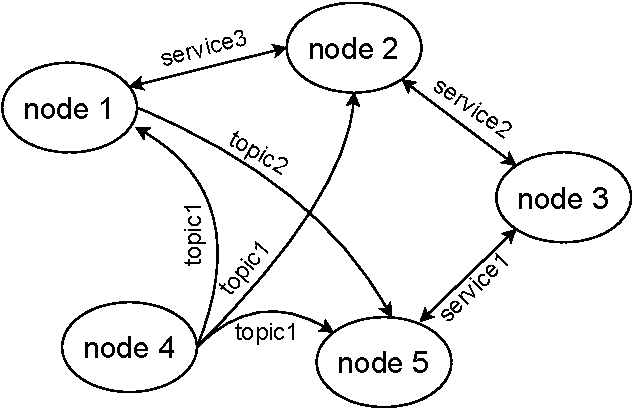
\includegraphics[width=\textwidth]{Figures/RosGraph.pdf}
    \end{column}
  \end{columns}
\end{frame}

\begin{frame}\frametitle{Tópicos y servicios}
  Los nodos (procesos) en ROS intercambian información a través de dos grandes patrones:
  \begin{columns}
    \begin{column}{0.6\textwidth}
        \begin{itemize}
        \item \textbf{Tópicos}
          \begin{itemize}
          \item Son un patrón $1:n$ de tipo \textit{publicador/suscriptor}
          \item Son no bloqueantes
          \item Utilizan estructuras de datos definidas en archivos \texttt{*.msg} para el envío de información
          \end{itemize}
        \item \textbf{Servicios}
          \begin{itemize}
          \item Son un patrón $1:1$ de tipo \textit{petición/respuesta}
          \item Son bloqueantes
          \item Utilizan estructuras de datos definidas en archivos \texttt{*.srv} para el intercambio de información. 
          \end{itemize}
        \end{itemize}
    \end{column}
    \begin{column}{0.4\textwidth}
      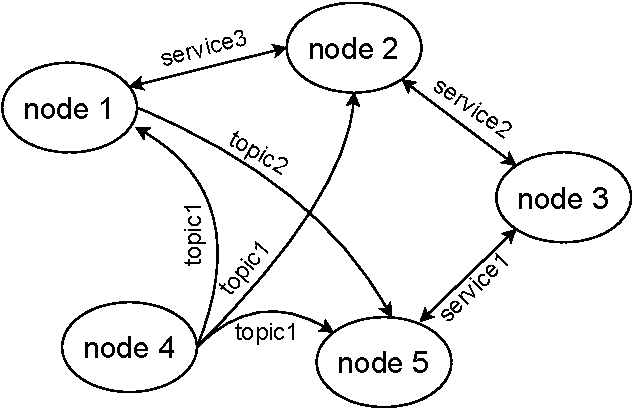
\includegraphics[width=\textwidth]{Figures/RosGraph.pdf}
    \end{column}
  \end{columns}
  \[\]
  Para mayor información:
  \begin{itemize}
  \item Tutoriales \url{http://wiki.ros.org/ROS/Tutorials}
  \item Koubâa, A. (Ed.). (2020). Robot Operating System (ROS): The Complete Reference. Springer Nature
  \end{itemize}
\end{frame}

\begin{frame}\frametitle{El simulador Gazebo}
  
\end{frame}

\begin{frame}[containsverbatim]\frametitle{Tarea 02 - La plataforma ROS}
  \begin{enumerate}
  \item Investigar aplicaciones de ROS y el simulador Gazebo. Se pueden consultar las siguientes páginas:
    \begin{itemize}
    \item https://www.openrobotics.org/markets
    \item https://vimeo.com/649649866/37198994b5
    \item https://robots.ros.org/robonaut2/
    \item https://github.com/nasa/astrobee
    \end{itemize}
  \item Buscar para qué sirven los comandos: \texttt{rosrun}, \texttt{rostopic list} y \texttt{rostopic echo}
  \item Abra el archivo \texttt{catkin\_ws/src/students/scripts/assignment02.py} y agregue el siguiente código en la línea 25:
    \begin{lstlisting}[language=Python,firstnumber=25]
n = int((msg.angle_max - msg.angle_min)/msg.angle_increment/2)
obstacle_detected = msg.ranges[n] < 1.0
  \end{lstlisting}
  En el mismo archivo, en la línea 45, agregue el siguiente código:
  \begin{lstlisting}[language=Python,firstnumber=45]
msg_cmd_vel = Twist()
msg_cmd_vel.linear.x = 0 if obstacle_detected else 0.3
pub_cmd_vel.publish(msg_cmd_vel)
  \end{lstlisting}
  \end{enumerate}
\end{frame}

\begin{frame}[containsverbatim]\frametitle{Tarea 02 - La plataforma ROS}
  \begin{enumerate}
    \setcounter{enumi}{3}
  \item Abra una terminal y corra la simulación con el comando (revise las instrucciones en el README del repositorio):
    \begin{verbatim}
   roslaunch surge_et_ambula justina_gazebo.launch
\end{verbatim}
  \item En otra terminal, corra la tarea 2 con el comando:
    \begin{verbatim}
   rosrun students assignment02.py
\end{verbatim}
  \item Observe el comportamiento y describa lo que sucede. De preferencia, elabore un diagrama de flujo que describa el comportamiento del robot.
  \end{enumerate}
  \[\]
  \textbf{Entregables:}
  \begin{itemize}
  \item Código modificado en la rama correspondiente del repositorio en línea.
  \item Documento escrito con todos los puntos anteriores. 
  \end{itemize}
  \textbf{Deadline: } 2023-08-31 al inicio de la clase. 
\end{frame}


